\documentclass[12pt,aspectratio=169,xcolor=dvipsnames]{beamer}
\usetheme{SimplePlus}
\usepackage{booktabs}
\usepackage{tikz}
\usepackage{pgfplots}
\usepackage{mathtools}

\usepackage{amsmath, amssymb}
\usepackage{tikz}

% Metadatos adaptados al contexto del curso
\title{Iteraciones, Puntos Fijos y Caos}
\subtitle{Aplicación: El Mapeo Logístico}
\author{Nicolás Barnafi}
\institute{Pontificia Universidad Católica de Chile \\ IMT1001 - Introducción a la Ingeniería Matemática}
\date{\today}

\begin{document}

\begin{frame}
    \titlepage
\end{frame}

\begin{frame}{Mapas de Punto Fijo}
    \begin{itemize}
        \item \textbf{Definición:} Sea $X$ un espacio normado y $T: X \to X$ un operador. Un punto $x^* \in X$ es un punto fijo de $T$ si:
        $$T(x^*) = x^*$$
        
        \item \textbf{Iteración de Picard:} Sucesión $\{x_n\}_{n \in \mathbb{N}}$ construida recursivamente dado un $x_0 \in X$:
        $$x_{n+1} = T(x_n)$$
        
        \item \textbf{Convergencia:} Si $T$ es una contracción (constante de Lipschitz $L < 1$), el Teorema del Punto Fijo de Banach asegura:
        \begin{enumerate}
            \item Existencia y unicidad de $x^*$.
            \item Convergencia asintótica: $\lim_{n \to \infty} x_n = x^*$.
        \end{enumerate}
    \end{itemize}
\end{frame}

\begin{frame}{Motivación: Dinámica Poblacional}
    \begin{itemize}
        \item Sea $P_n$ la población en el instante $n$.
        \item \textbf{Crecimiento sin restricciones:} Tasa de crecimiento $R > 0$.
        $$P_{n+1} = R P_n$$
        
        \item \textbf{Capacidad de carga:} Recursos limitados, capacidad máxima $K > 0$. Se atenúa el crecimiento por el factor $(1 - P_n / K)$.
        
        \item \textbf{Modelo discreto de Verhulst:}
        $$P_{n+1} = R P_n \left(1 - \frac{P_n}{K}\right)$$
        
        \item \textbf{Mapeo Logístico:} Normalizando variables con $x_n = P_n / K$:
        $$x_{n+1} = r x_n (1 - x_n) = T(x_n)$$
    \end{itemize}
\end{frame}

\begin{frame}{Puntos Fijos del Mapeo Logístico}

        $$x_{n+1} = r x_n (1 - x_n) = T(x_n)$$

        \idea{Calcular puntos fijos}

        \idea{Encontrar $r$ tal que $T$ sea contracción.}
\end{frame}

\begin{frame}{Puntos Fijos del Mapeo Logístico}
    \begin{itemize}
        \item Sea $f(x) = r x (1 - x)$. Puntos fijos satisfacen la ecuación de balance:
        $$r x^* (1 - x^*) = x^* \implies x^*(r - r x^* - 1) = 0$$
        
        \item \textbf{Raíces (Puntos Fijos):}
        $$x_1^* = 0, \quad x_2^* = 1 - \frac{1}{r}$$
        
        \item \textbf{Condición de Estabilidad local:} Teorema del Punto Fijo requiere un operador localmente contractante.
        $$|f'(x^*)| < 1$$
        
        \item \textbf{Derivada funcional:}
        $$f'(x) = r(1 - 2x)$$
    \end{itemize}
\end{frame}

\begin{frame}{Caracterización del Régimen Contractante}
    \begin{itemize}
        \item \textbf{Estabilidad en $x_1^* = 0$:}
        $$|f'(0)| = |r| < 1 \implies \text{Atractor para } r \in (0,1)$$
        
        \item \textbf{Estabilidad en $x_2^* = 1 - \frac{1}{r}$:}
        $$|f'(x_2^*)| = \left|r \left(1 - 2\left(1 - \frac{1}{r}\right)\right)\right| = |2 - r|$$
        
        \item \textbf{Condición de contracción para $x_2^*$:}
        $$|2 - r| < 1 \implies -1 < 2 - r < 1$$
        $$\implies 1 < r < 3$$
        
        \item \textbf{Corolario:} Para $r \in (1,3)$, la iteración de Picard converge a $x_2^*$. Para $r > 3$, se pierde la garantía de contracción (bifurcación y caos).
    \end{itemize}
\end{frame}

\begin{frame}{Diagrama de Telaraña (Cobweb Map)}
        \textbf{Definición:} Construcción geométrica de la órbita $\{x_n\}_{n \in \mathbb{N}}$ generada por el sistema dinámico discreto $x_{n+1} = f(x_n)$.
            \begin{columns}
                \begin{column}{0.45\textwidth}
                    \begin{itemize}
                        \item \textbf{Algoritmo iterativo:}
                            $$ (x_n, 0) \xrightarrow{} (x_n, f(x_n)) \xrightarrow{} (x_{n+1}, x_{n+1}) $$
                        \item \textbf{Ejemplo:} Mapeo logístico convergente, $f(x) = 2.8x(1-x)$, con condición inicial $x_0 = 0.1$.
                    \end{itemize}

                    \vspace{0.2cm}
                \end{column}
            \begin{column}{0.45\textwidth}
                %\begin{center}
                    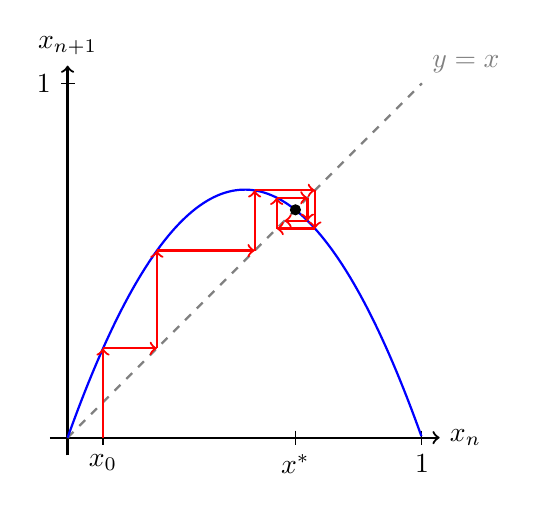
\begin{tikzpicture}[scale=4.5]
                        % Ejes
                        \draw[->, thick] (-0.05, 0) -- (1.05, 0) node[right] {$x_n$};
                        \draw[->, thick] (0, -0.05) -- (0, 1.05) node[above] {$x_{n+1}$};

                        % Ticks importantes
                        \draw (0.643, 0.02) -- (0.643, -0.02) node[below] {$x^*$};
                        \draw (0.1, 0.02) -- (0.1, -0.02) node[below] {$x_0$};
                        \draw (0.02, 1) -- (-0.02, 1) node[left] {$1$};
                        \draw (1, 0.02) -- (1, -0.02) node[below] {$1$};

                        % Identidad y = x
                        \draw[dashed, thick, gray] (0,0) -- (1,1) node[above right, text=gray] {$y=x$};

                        % Función Logística f(x) = 2.8*x*(1-x)
                        \draw[thick, blue, domain=0:1, samples=100] plot (\x, {2.8*\x*(1-\x)}); % node[pos=0.8, above right, font=\tiny] {$f(x)$};

                        % Iteraciones (Telaraña)
                        % x0 = 0.1, f(x0) = 0.252
                        \draw[->, red, thick] (0.1, 0) -- (0.1, 0.252);
                        \draw[->, red, thick] (0.1, 0.252) -- (0.252, 0.252);

                        % x1 = 0.252, f(x1) = 0.528
                        \draw[->, red, thick] (0.252, 0.252) -- (0.252, 0.528);
                        \draw[->, red, thick] (0.252, 0.528) -- (0.528, 0.528);

                        % x2 = 0.528, f(x2) = 0.698
                        \draw[->, red, thick] (0.528, 0.528) -- (0.528, 0.698);
                        \draw[->, red, thick] (0.528, 0.698) -- (0.698, 0.698);

                        % x3 = 0.698, f(x3) = 0.590
                        \draw[->, red, thick] (0.698, 0.698) -- (0.698, 0.590);
                        \draw[->, red, thick] (0.698, 0.590) -- (0.590, 0.590);

                        % x4 = 0.590, f(x4) = 0.677
                        \draw[->, red, thick] (0.590, 0.590) -- (0.590, 0.677);
                        \draw[->, red, thick] (0.590, 0.677) -- (0.677, 0.677);

                        % x5 = 0.677, f(x5) = 0.612
                        \draw[->, red, thick] (0.677, 0.677) -- (0.677, 0.612);
                        \draw[->, red, thick] (0.677, 0.612) -- (0.612, 0.612);

                        % Punto fijo intersección
                        \filldraw[black] (0.643, 0.643) circle (0.4pt);
                    \end{tikzpicture}
            %\end{center}
        \end{column}
    \end{columns}
\end{frame}

\end{document}
